\documentclass[11pt,letterpaper]{article}
\usepackage[left=1.00in, right=1.00in, top=1.00in, bottom=1.00in]{geometry}
\usepackage{titling}
\usepackage{amsmath} % Advanced math typesetting. use equation environment
\usepackage[numbered,framed]{matlab-prettifier} % Used for MATLAB code
\usepackage{listings}
\usepackage{mathtools}
\usepackage{amsbsy}
\usepackage{bm}
\usepackage{graphicx} % Add pictures to your document. use figure environment
\usepackage{subcaption} % Add multiple images in one location. use subfigure environment
\usepackage{amssymb} % For real numbers R symbol
\usepackage{grffile}
\usepackage{hyperref} % For web links
\begin{document}
	
	% ========== Edit title here(For help: http://ctan.mirrors.hoobly.com/macros/latex/contrib/titling/titling.pdf)
	\setlength{\droptitle}{-1in} % Eliminate the default vertical space
	\pretitle{\begin{center}\LARGE}
		\title{Duckiebot Lane Follower with Convolutional Neural Networks\\- Progress Report 1 -}
		\posttitle{\par\end{center}}
	\preauthor{\begin{center}}
		\author{{\Large Burak Aksoy}\\
			aksoyb2@rpi.edu}
		\postauthor{\par\end{center}}
	
	%\predate{}
	%\postdate{}
	%\date{}
	\date{May 15, 2019} 

	\maketitle
	
	\noindent\makebox[\linewidth]{\rule{\linewidth}{2pt}}
	
	\tableofcontents
	
	% ========== Begin report Details here
	\section{Introduction}
	\subsection{Lane Following Algorithm Overview}
	Duckiebot project already has a Lane Following algorithm which takes the camera images, detects lines, calculates its position and orientation in the lane, apply some control dynamics, decides required linear and angular velocity, and sets the wheel speeds accordingly. Lane Following algorithm overview flow can be seen in Figure \ref{fig:01}. 
	
	\begin{figure}[h!]
		\centering
		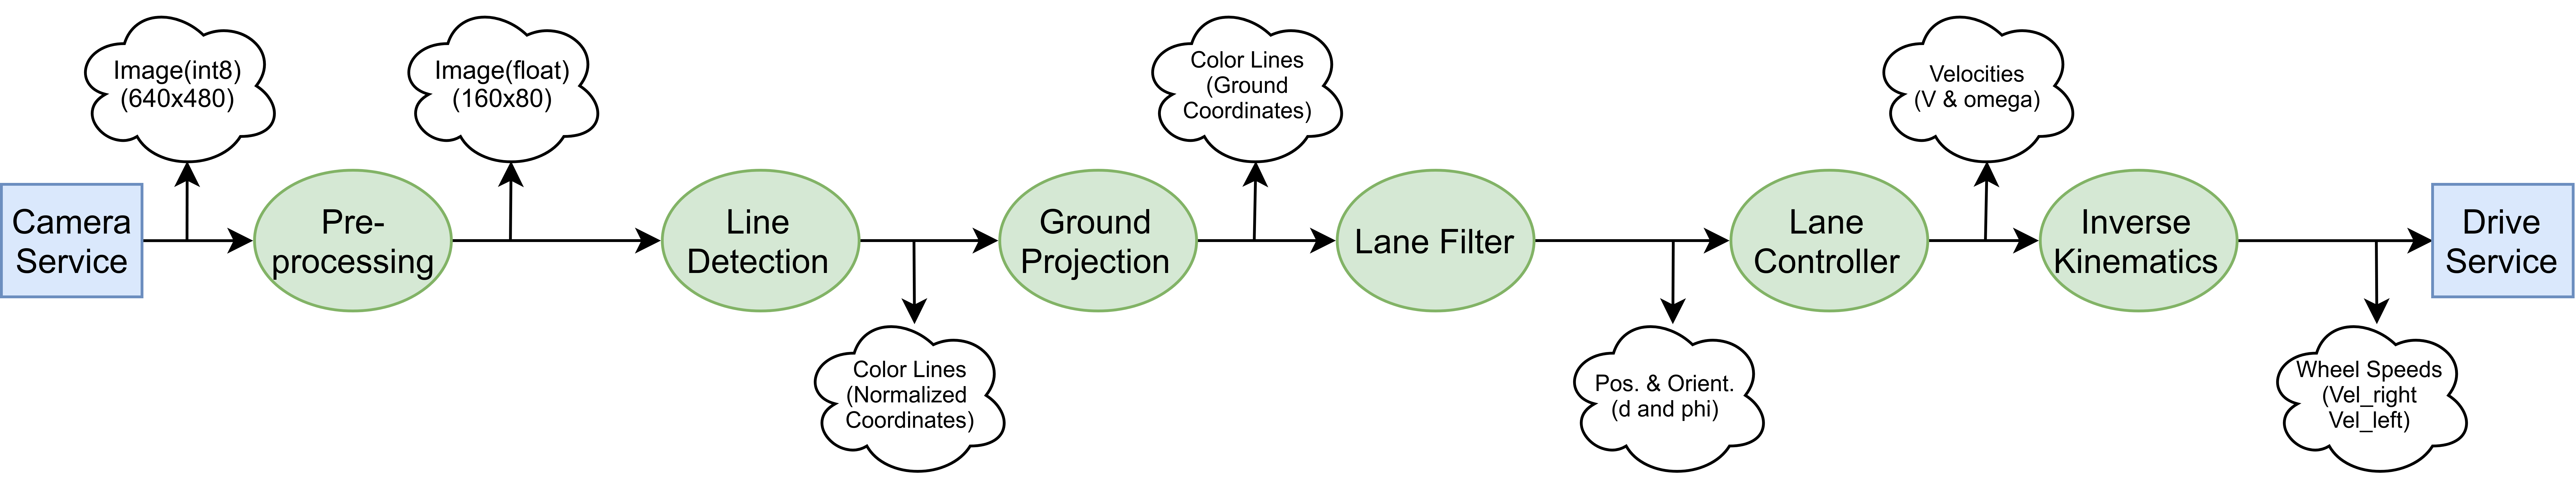
\includegraphics[width=1.0\linewidth]{algo0.png}
		\caption{Lane Following algorithm overview flow.}
		\label{fig:01}
	\end{figure}
	
	This algorithm is already implemented in Robotic Opereating System(ROS) using Python. The source files can be found in \href{https://github.com/rpiRobotics/duckietown/tree/master/catkin_ws/src}{RPI Robotics Duckietown GitHub repository}. 
	
	In our previous work, we have implemented the same algorithm also in \href{https://robotraconteur.com/}{Robot Raconteur}(RR) framework using Python. The source files can be found in \href{https://github.com/burakaksoy/DuckiebotRR}{in this link}.  
	
	We compared the performance results of ROS and RR experimenting on a Duckiebot powered with \href{https://www.raspberrypi.org/products/raspberry-pi-2-model-b/}{Raspberry Pi 2 Model B} and observed average rate of completing the algorithm as in Table \ref{table:1}
	
	\begin{table}[h!]
	\centering
	\begin{tabular}{||c c||} 
		\hline
		Framework & Rate(per second) \\ [0.5ex] 
		\hline\hline
		ROS &  9.5\\ 
		\hline
		RR & 11.0  \\
		\hline
	\end{tabular}
	\caption{Performance comparison between RR and ROS}
	\label{table:1}
	\end{table}
	
	The obtained result shows that RR gives approximately 1.5 completion rate per second faster response than ROS. This gain is mainly result of fast Camera and Drive Service that RR provides (Rectangular, blue backgrounded steps in Figure \ref{fig:01}). Other steps of the algorithm (Elliptic, green backgrounded steps in Figure \ref{fig:01}) are basically gives the same performance due to using the same programming language and code on the same machine.
	
	\subsection{Deep Learning Idea}
	
	Our next aim is improving the performance of these steps eliminating them and instead, using a Deep Learning approach with a trained model. We use a Convolutional Neural Network(CNN) since we are dealing with images and our model will solve a regression problem since we are generating continuous messages rather than classification. Since Raspberry Pi 2 Model B is not powerful enough for a deep learning image processing, we  use \href{https://movidius.github.io/ncsdk/ncs.html}{Intel Movidius Neural Compute Stick} for trained model inferences from camera images. After creating a Duckietown map as in Figure \ref{fig:02} and let the Duckiebot travel in this map using the already implemented RR lane following algorithm, data is collected with saving the camera images and corresponding control messages into external memory. 
	
	\begin{figure}[h!]
		\centering
		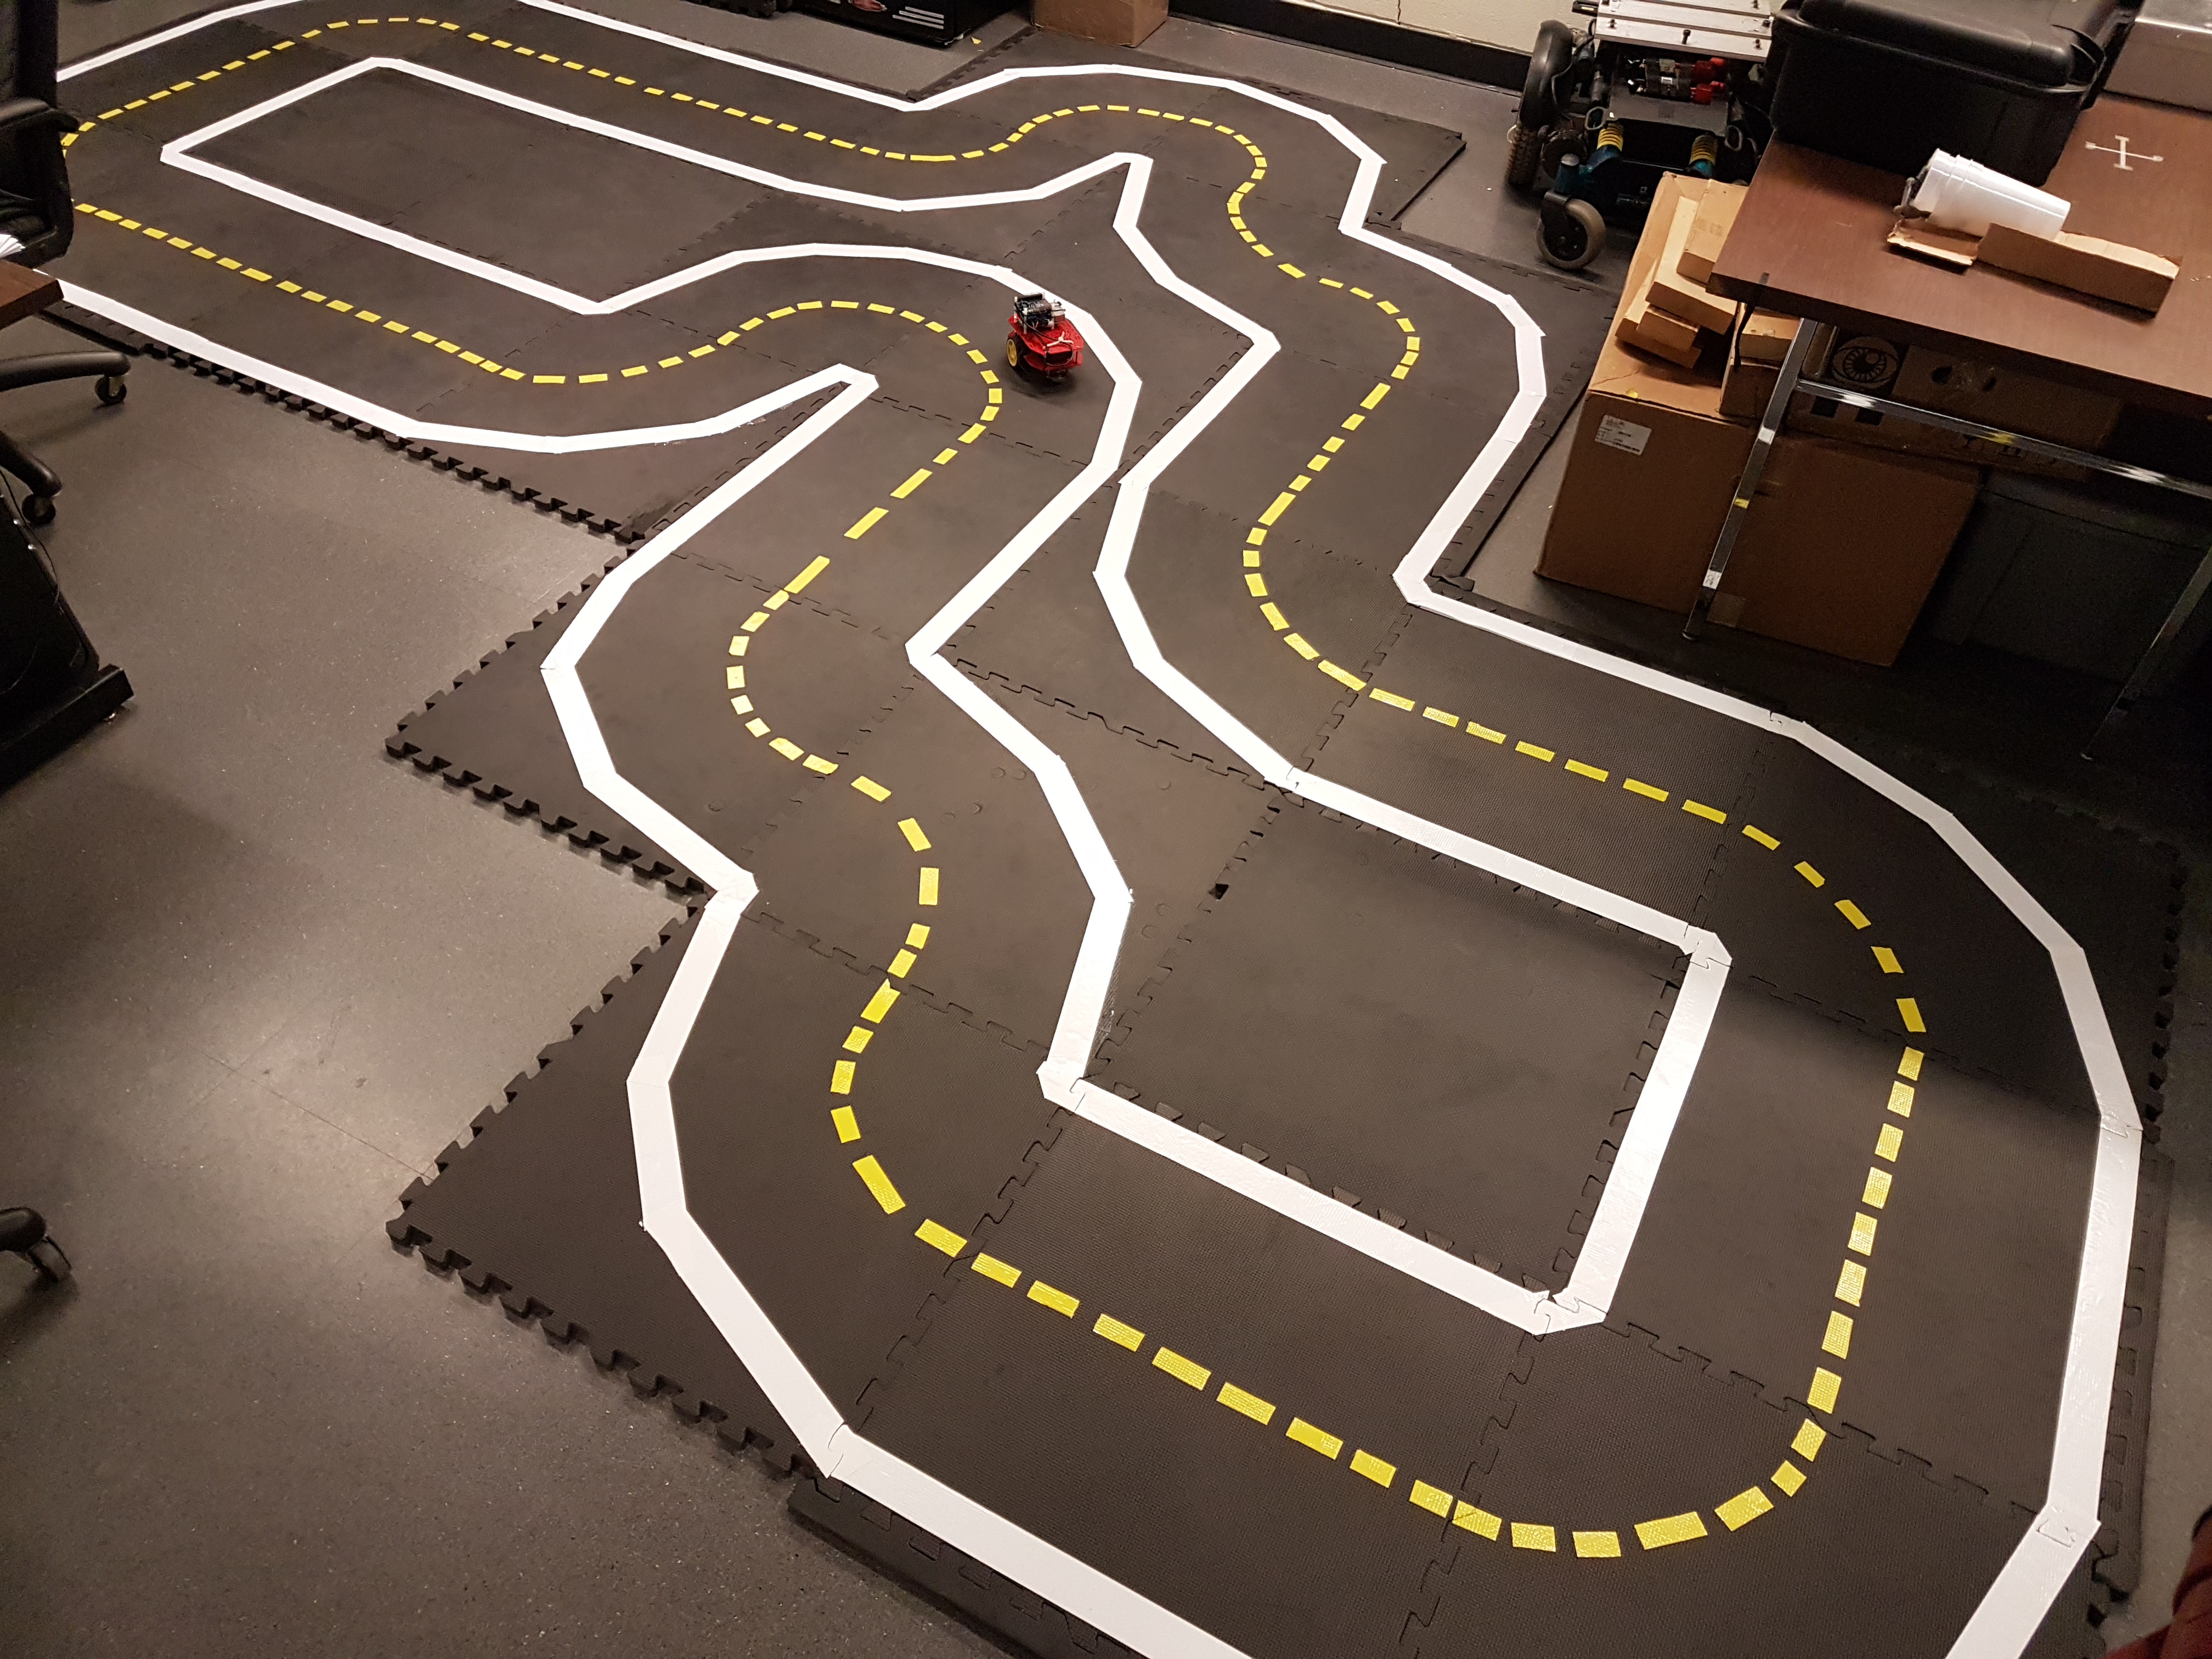
\includegraphics[width=0.7\linewidth]{map.jpg}
		\caption{Training Map.}
		\label{fig:02}
	\end{figure}
	
	\section{Training Approach 1: Predict $d$ and $\phi$ from Image}
	Please see Figure \ref{fig:03} to visualize this approach.  
	
	\begin{figure}[h!]
		\centering
		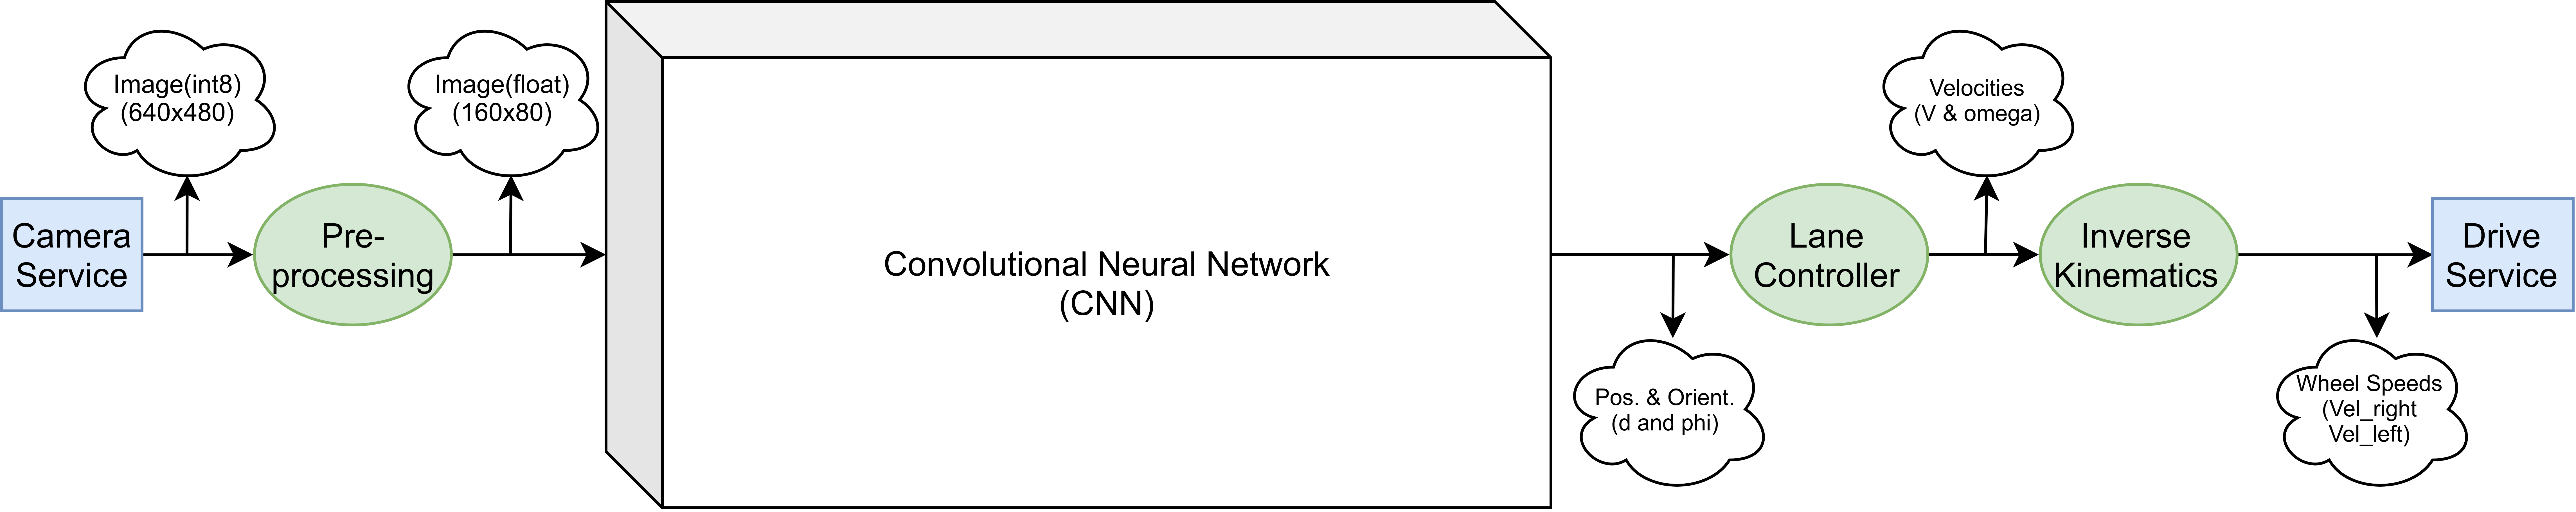
\includegraphics[width=1.1\linewidth]{algo1.png}
		\caption{Lane Following algorithm overview flow with 1st Approach CNN.}
		\label{fig:03}
	\end{figure}
	
	This kind of approach replaces some relatively heavy steps such as Line detection, Ground Projection and Lane Filter steps from the algorithm flow with a trained CNN model and predicts position $d$ in range (-0.15,0.30) meters and orientation $\phi$ in range (-1.5,1.5) radian errors with respect to lane as a regression problem. The reason behind choosing this idea first, rather than an end-to-end approach, is that extracting only $d$ and $\phi$ information can give more flexibility in terms of controller and setting different speed values for the robot which might be useful for later applications.
	
	\subsection{Training Data}
	Data for this approach has 9010 colored(3 channel) images in total with size 160x80. Data is divided as 8000 training and 1010 validation images, and they are labeled with their corresponding $d$ and $\phi$ values. Some sample images from data can be seen on Figure \ref{fig:04}.   
	
 \begin{figure}[h!]
 	\centering
 	\begin{subfigure}[b]{0.24\linewidth}
 		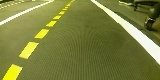
\includegraphics[width=\linewidth]{00008.jpg}
 		\caption{$d=-0.03,\ \phi=,0.0$}
 	\end{subfigure}
 	\begin{subfigure}[b]{0.24\linewidth}
 		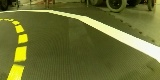
\includegraphics[width=\linewidth]{00251.jpg}
 		\caption{$d=0.03,\ \phi=-0.55$}
 	\end{subfigure}
 	\begin{subfigure}[b]{0.24\linewidth}
 		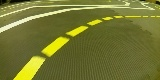
\includegraphics[width=\linewidth]{00342.jpg}
 		\caption{$d=-0.05,\ \phi=0.7$}
 	\end{subfigure}
 	\begin{subfigure}[b]{0.24\linewidth}
 		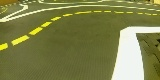
\includegraphics[width=\linewidth]{00504.jpg}
 		\caption{$d=-0.11,\ \phi=0.4$}
 	\end{subfigure}
 	\begin{subfigure}[b]{0.24\linewidth}
 		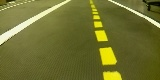
\includegraphics[width=\linewidth]{00653.jpg}
 		\caption{$d=0.13,\ \phi=0.1$}
 	\end{subfigure}
 	\begin{subfigure}[b]{0.24\linewidth}
 		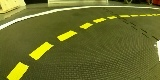
\includegraphics[width=\linewidth]{05842.jpg}
 		\caption{$d=-0.05,\ \phi=0.65$}
 	\end{subfigure}
 	\begin{subfigure}[b]{0.24\linewidth}
 		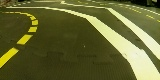
\includegraphics[width=\linewidth]{06071.jpg}
 		\caption{$d=-0.03,\ \phi=0.05$}
 	\end{subfigure}
 	\begin{subfigure}[b]{0.24\linewidth}
 		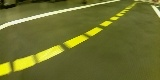
\includegraphics[width=\linewidth]{06370.jpg}
 		\caption{$d=-0.07,\ \phi=0.75$}
 	\end{subfigure}
 	\caption{Some sample training images and their labels.}
 	\label{fig:04}
 \end{figure} 
	
	This data obtained saving the images when Duckiebot travel in the map three loops in one direction and three loops in the other direction. 3483 images are saved during a relatively faster travel to capture the larger $d$ and $\phi$ values and 5527 images are saved during a normal speed travel.
	
	\subsection{CNN Architecture 1}
	Overall, The first implemented architecture (CNN Architecture 1) takes 160x80x3 images as input and has 4 convolutional layers with filter sizes (7x7x3x16), (5x5x16x32), (5x5x32x64), (5x5x64x64) respectively. Each convolution layer is followed by a Max-Pooling layer with a window size (2x2) with stride 2. After convolution and max-pooling layers, tensor is flattened to a vector with length 3200. A fully connected layer is added with size 1024 and then $d$ and $\phi$ is calculated as output. A visualization of this architecture can be seen on Figure \ref{fig:05}
	
	\begin{figure}[h!]
		\centering
		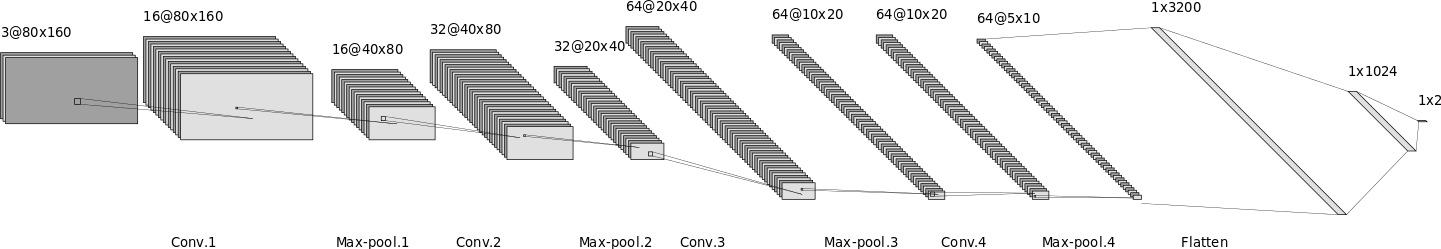
\includegraphics[width=1.0\linewidth]{arc1.png}
		\caption{CNN Architecture 1 Visualization.}
		\label{fig:05}
	\end{figure}
	
	\subsubsection{CNN Architecture 1: Error Results}
	Obtained training results of CNN Architecture 1 in terms of validation data average error values in $d$ and $\phi$ with respect to epochs passed can be seen at left of figure \ref{fig:06}. the right side of the Figure \ref{fig:06} shows resulted error values. Based on these results, we obtained in average $3.25$ cm error in $d$ and $6.45$ degree error in $\phi$ for prediction from the camera images. 
	
	\begin{figure}[h!]
		\centering
		\begin{subfigure}[b]{0.74\linewidth}
			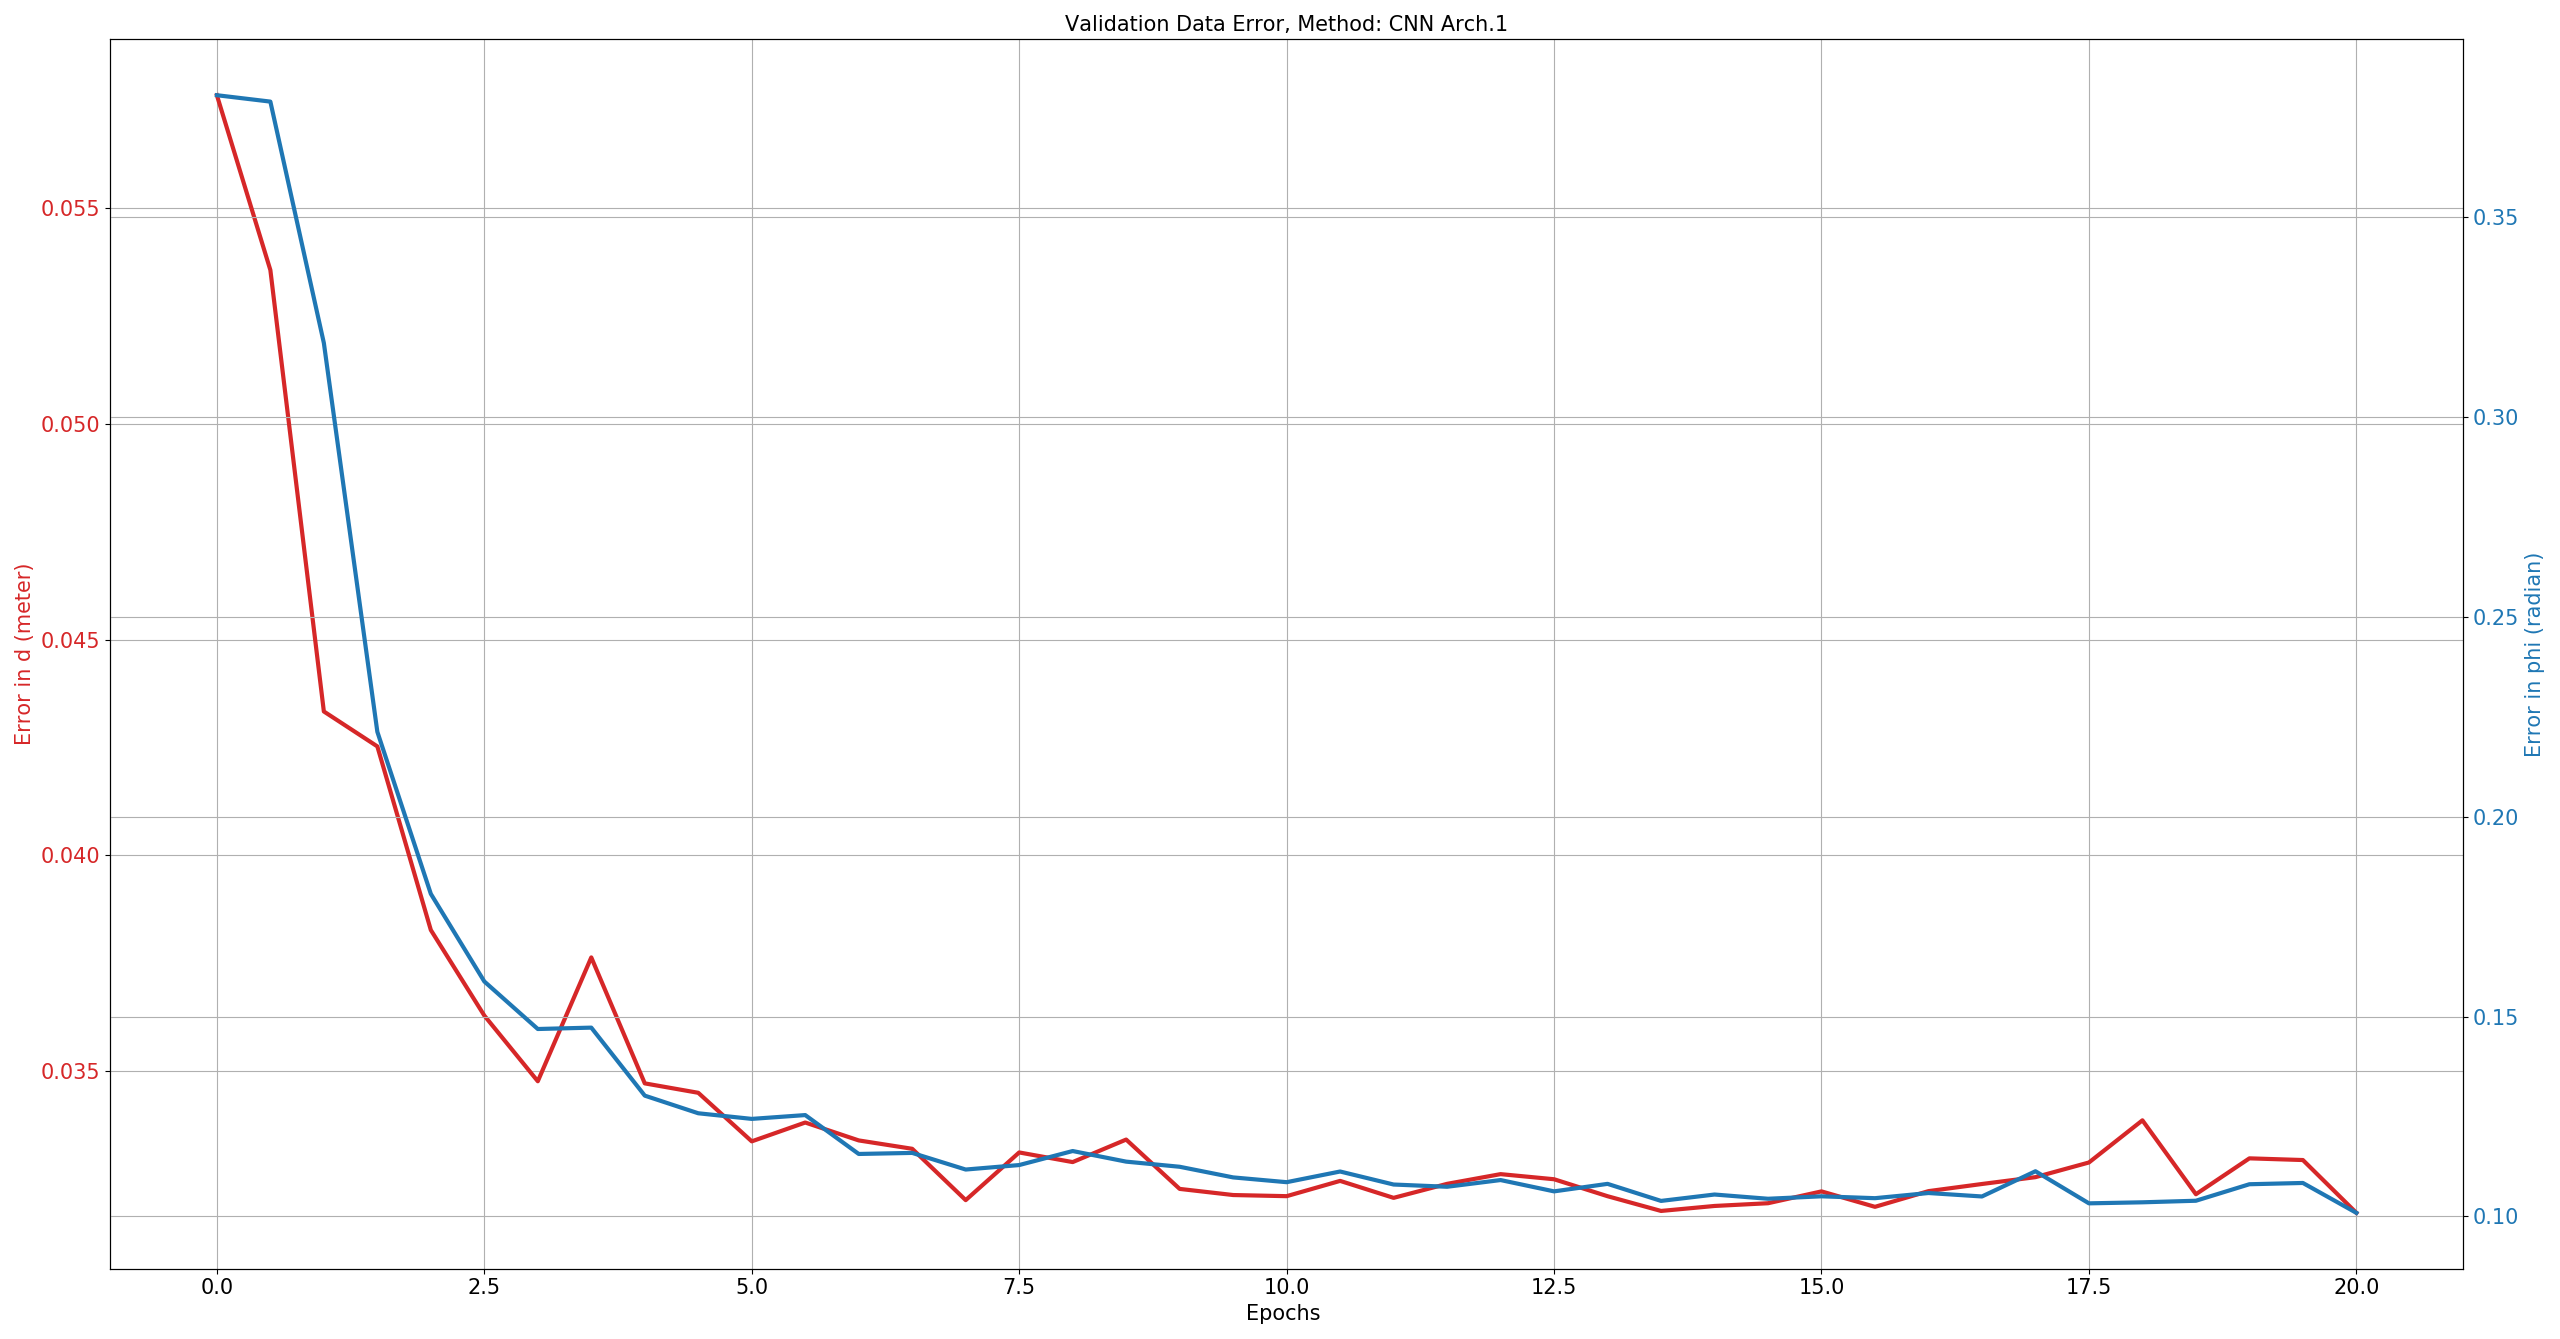
\includegraphics[width=\linewidth]{err-arc1.png}
			\caption{Errors wrt. Epochs}
		\end{subfigure}
		\begin{subfigure}[b]{0.24\linewidth}
			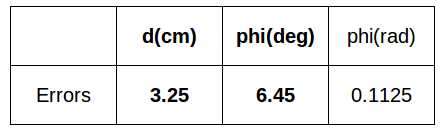
\includegraphics[width=\linewidth]{err-arc1-table.png}
			\caption{Resulted Errors}
		\end{subfigure}
		\caption{Validation Data Errors with CNN Architecture 1}
		\label{fig:06}
	\end{figure}  
	
	\subsubsection{CNN Architecture 1: Timing Results}
	Since we are trying to improve the performance of algorithm, it is important to see the timing results of Lane following algorithm with CNN and compare it with the existing RR performances. What we observe from Figure \ref{fig:07} is that we decreased the loop time by approximately 4.5 ms which is not a sufficient improvement considering the error results. In the next section, we will examine another CNN architecture to decrease the inference time of the CNN model without increasing the error rates. 
	
	\begin{figure}[h!]
		\centering
		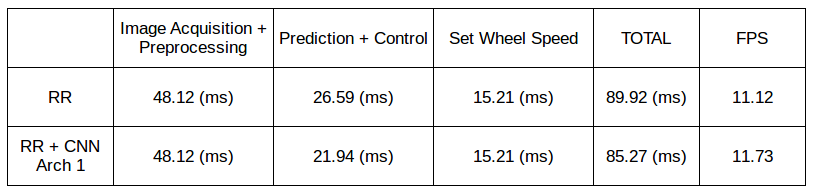
\includegraphics[width=0.7\linewidth]{time-arc1.png}
		\caption{CNN Architecture 1 Timing Performance.}
		\label{fig:07}
	\end{figure}
	
	\subsection{CNN Architecture 2}
	With our new CNN architecture we built a simpler model. Overall, our new architecture (CNN Architecture 2) again takes 160x80x3 images as input and has 4 convolutional layers with filter sizes (7x7x3x16), (5x5x16x32), (5x5x32x64), (5x5x64x64) respectively. This time, however, convolution layers are not followed by Max-Pooling layers. Instead, we will apply convolutions with stride 2 and the obtained tensor sizes will be the same. After  strided convolution layers, the tensor again flattened to a vector with length 3200. A fully connected layer is added with size 1024 and then $d$ and $\phi$ is calculated as output. A visualization of new simpler architecture can be seen on Figure \ref{fig:08}
	
	\begin{figure}[h!]
		\centering
		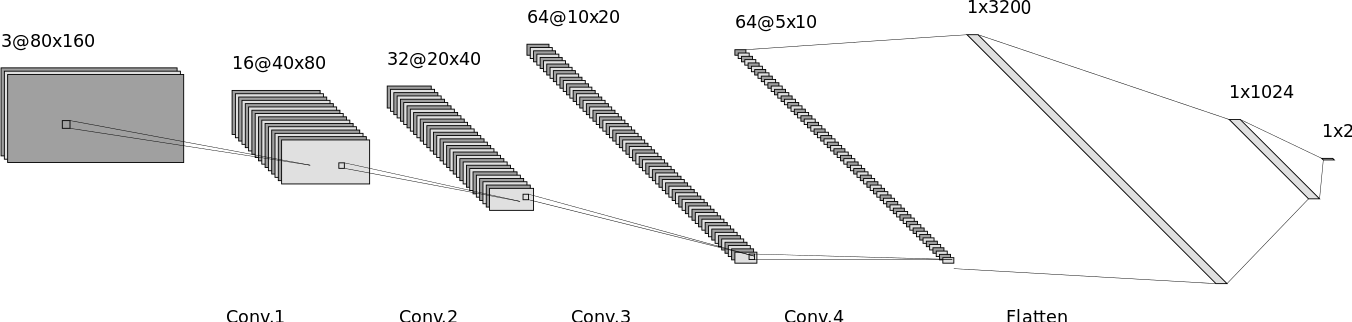
\includegraphics[width=1.0\linewidth]{arc2.png}
		\caption{CNN Architecture 2 Visualization.}
		\label{fig:08}
	\end{figure}
	
	\subsubsection{CNN Architecture 2: Error Results}
	Obtained training results of CNN Architecture 2 in terms of validation data average error values in $d$ and $\phi$ with respect to epochs passed can be seen at left of figure \ref{fig:09}. the right side of the Figure \ref{fig:09} shows resulted error values. Based on these results, we obtained in average $3.11$ cm error in $d$ and $7.34$ degree error in $\phi$ for prediction from the camera images. Compared with the previous architecture, this one performed slighlty better in $d$ and slightly worse in $\phi$. Therefore, the timing performance will be more decisive for which one to be used.  
	
	\begin{figure}[h!]
		\centering
		\begin{subfigure}[b]{0.74\linewidth}
			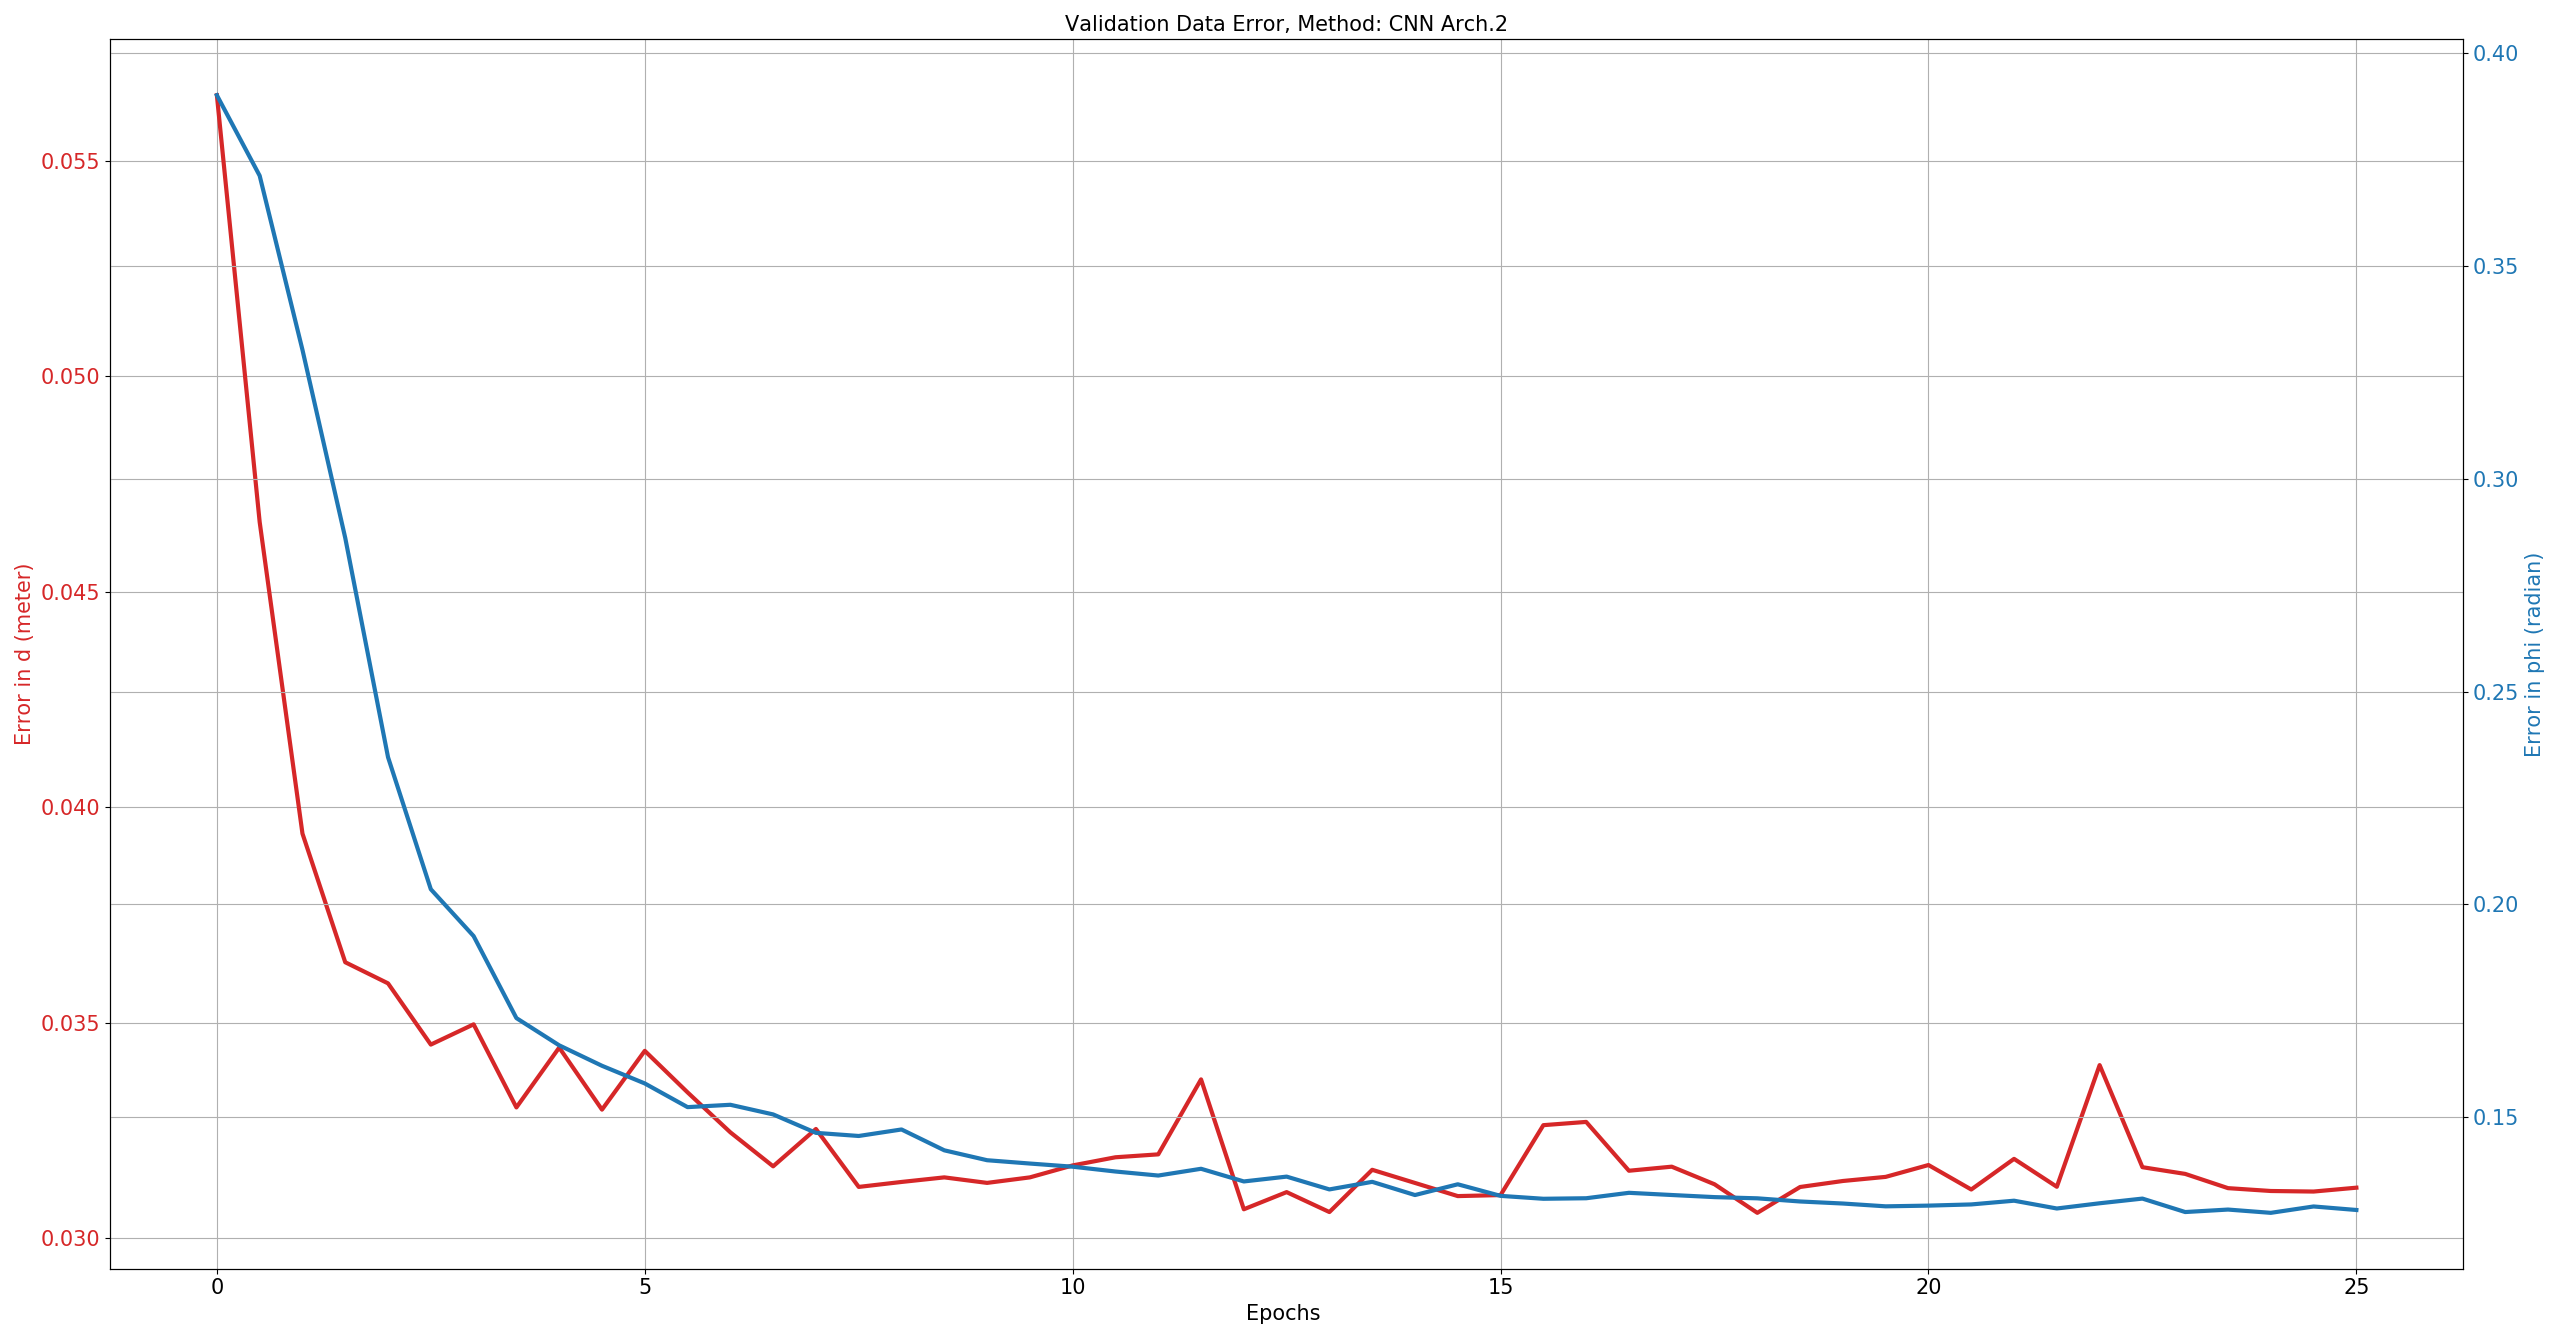
\includegraphics[width=\linewidth]{err-arc2.png}
			\caption{Errors wrt. Epochs}
		\end{subfigure}
		\begin{subfigure}[b]{0.24\linewidth}
			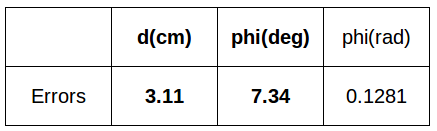
\includegraphics[width=\linewidth]{err-arc2-table.png}
			\caption{Resulted Errors}
		\end{subfigure}
		\caption{Validation Data Errors with CNN Architecture 2}
		\label{fig:09}
	\end{figure}  
	
	\subsubsection{CNN Architecture 2: Timing Results}
	Since we are trying to improve the performance of algorithm, it is important to see the timing results of Lane following algorithm with CNN and compare it with the existing RR performances. What we observe from Figure \ref{fig:10} is that we decreased the loop time by approximately 10.5 ms with respect to RR and approximately 6 ms with respect to CNN Arch.1. Since this result with 12.6 FPS can be considered as a performance improvement for our system, we decided to use CNN Architecture 2.
	
	\begin{figure}[h!]
		\centering
		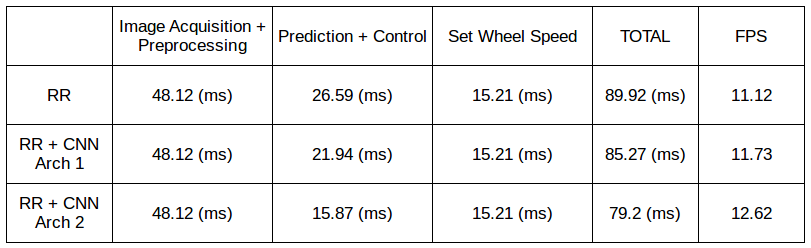
\includegraphics[width=0.7\linewidth]{time-arc2.png}
		\caption{CNN Architecture 2 Timing Performance.}
		\label{fig:10}
	\end{figure}
	
	\subsection{Real World Experimentation with Training Approach 1}
	Until now, we mainly focused on finding the best possible fast and accurate CNN model without actual experimenting the lane following algorithm with CNN. Using the discussed models above, we let the Duckibot travel, however none of the models with Training Approach 1 did not perform a sufficiently successful lane following.
	
	In the next section, we will modify our training approach to a new one.
	
	\section{Training Approach 2 (End-to-end): Predict $V_{left}$ and $V_{right}$ from Image}
	Please see Figure \ref{fig:11} to visualize this approach.  
	
	\begin{figure}[h!]
		\centering
		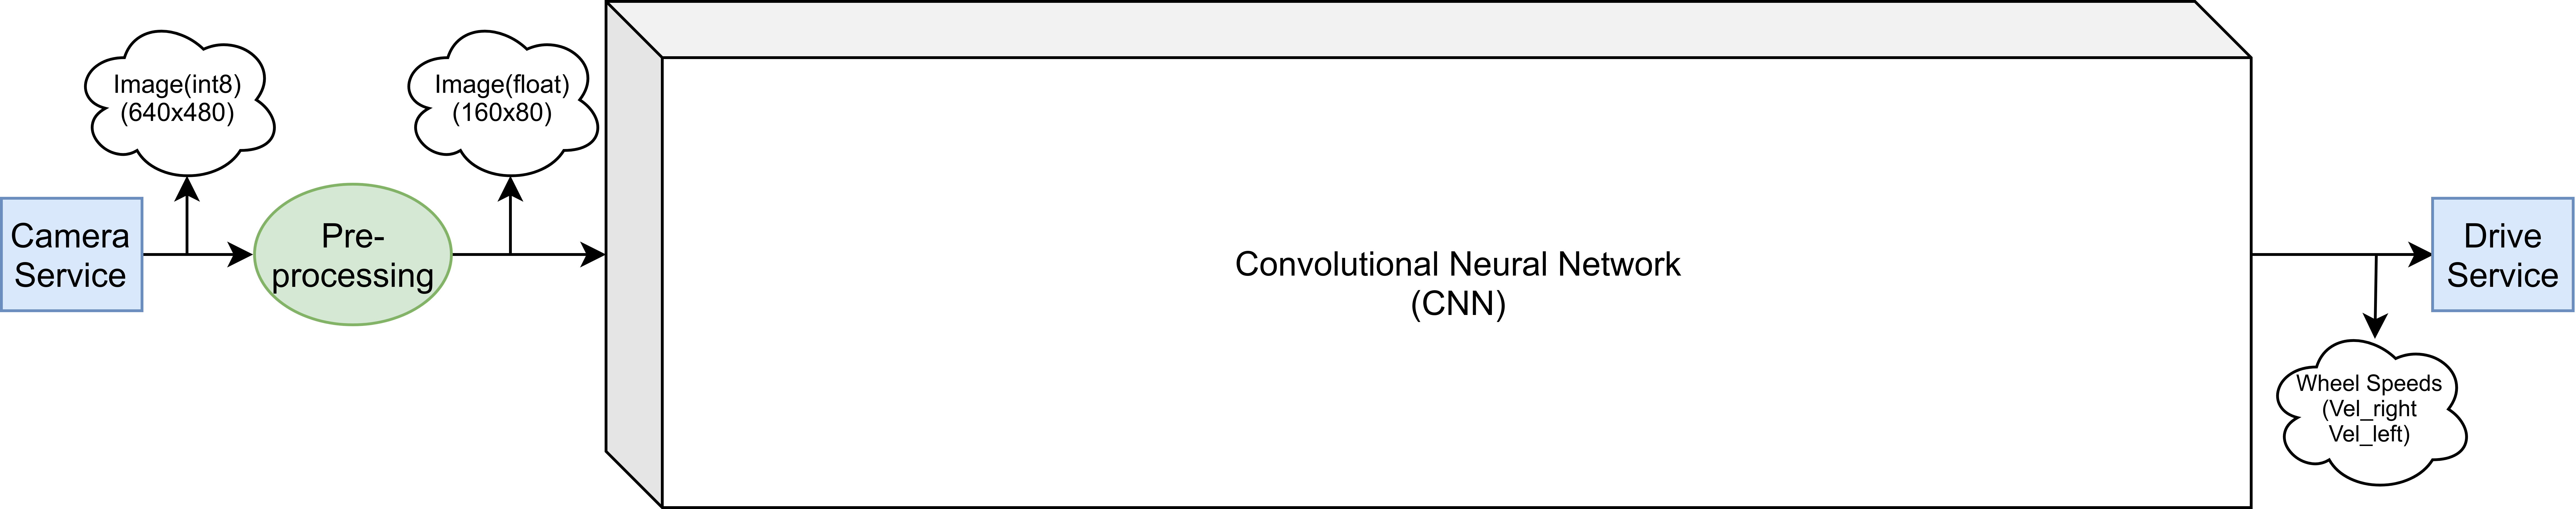
\includegraphics[width=1.1\linewidth]{algo2.png}
		\caption{Lane Following algorithm overview flow with 2nd Approach CNN.}
		\label{fig:11}
	\end{figure}
	
	This approach replaces Lane Controller and Inverse Kinematics steps in addition to the relatively heavy in the previous approach. Algorithm flow with a trained CNN model and predicts $V_{left}$ and $V_{right}$ values both in range $(-14, 58)$ for our training data as a regression problem. Speed value $100$ means full speed of the wheels in forward direction and $-100$ means full speed in the reverse direction. Neutral going forward speed is approximately $22.5$. Mean and standard deviation of whole speed data for $V_{left}$ and $V_{right}$ are observed as $22.5$ and $10.2$ respectively.
	
	\subsection{Training Data}
	Data for this approach has 5378 colored(3 channel) images in total with size 160x80. Data is divided as 4950 training and 428 validation images, and they are labeled with their corresponding $V_{left}$ and $V_{right}$ values.
	
	This data obtained saving the images when Duckiebot travel in the map three loops in one direction and three loops in the other direction. In this approach since we are directly learning the required wheel speeds, all data saved during normal speed travel.
	
	\subsection{Approach 2: CNN Architecture}
	We will use CNN Architecture 2 examined in the previous section due to its observed time performance improvement.
	
	\subsubsection{Approach 2: Error Results}
	Obtained training results of Approach 2 in terms of validation data average error values in $V_{left}$ and $V_{right}$ with respect to epochs passed can be seen at left of figure \ref{fig:12}. the right side of the Figure \ref{fig:12} shows resulted error values.
	
	\begin{figure}[h!]
		\centering
		\begin{subfigure}[b]{0.84\linewidth}
			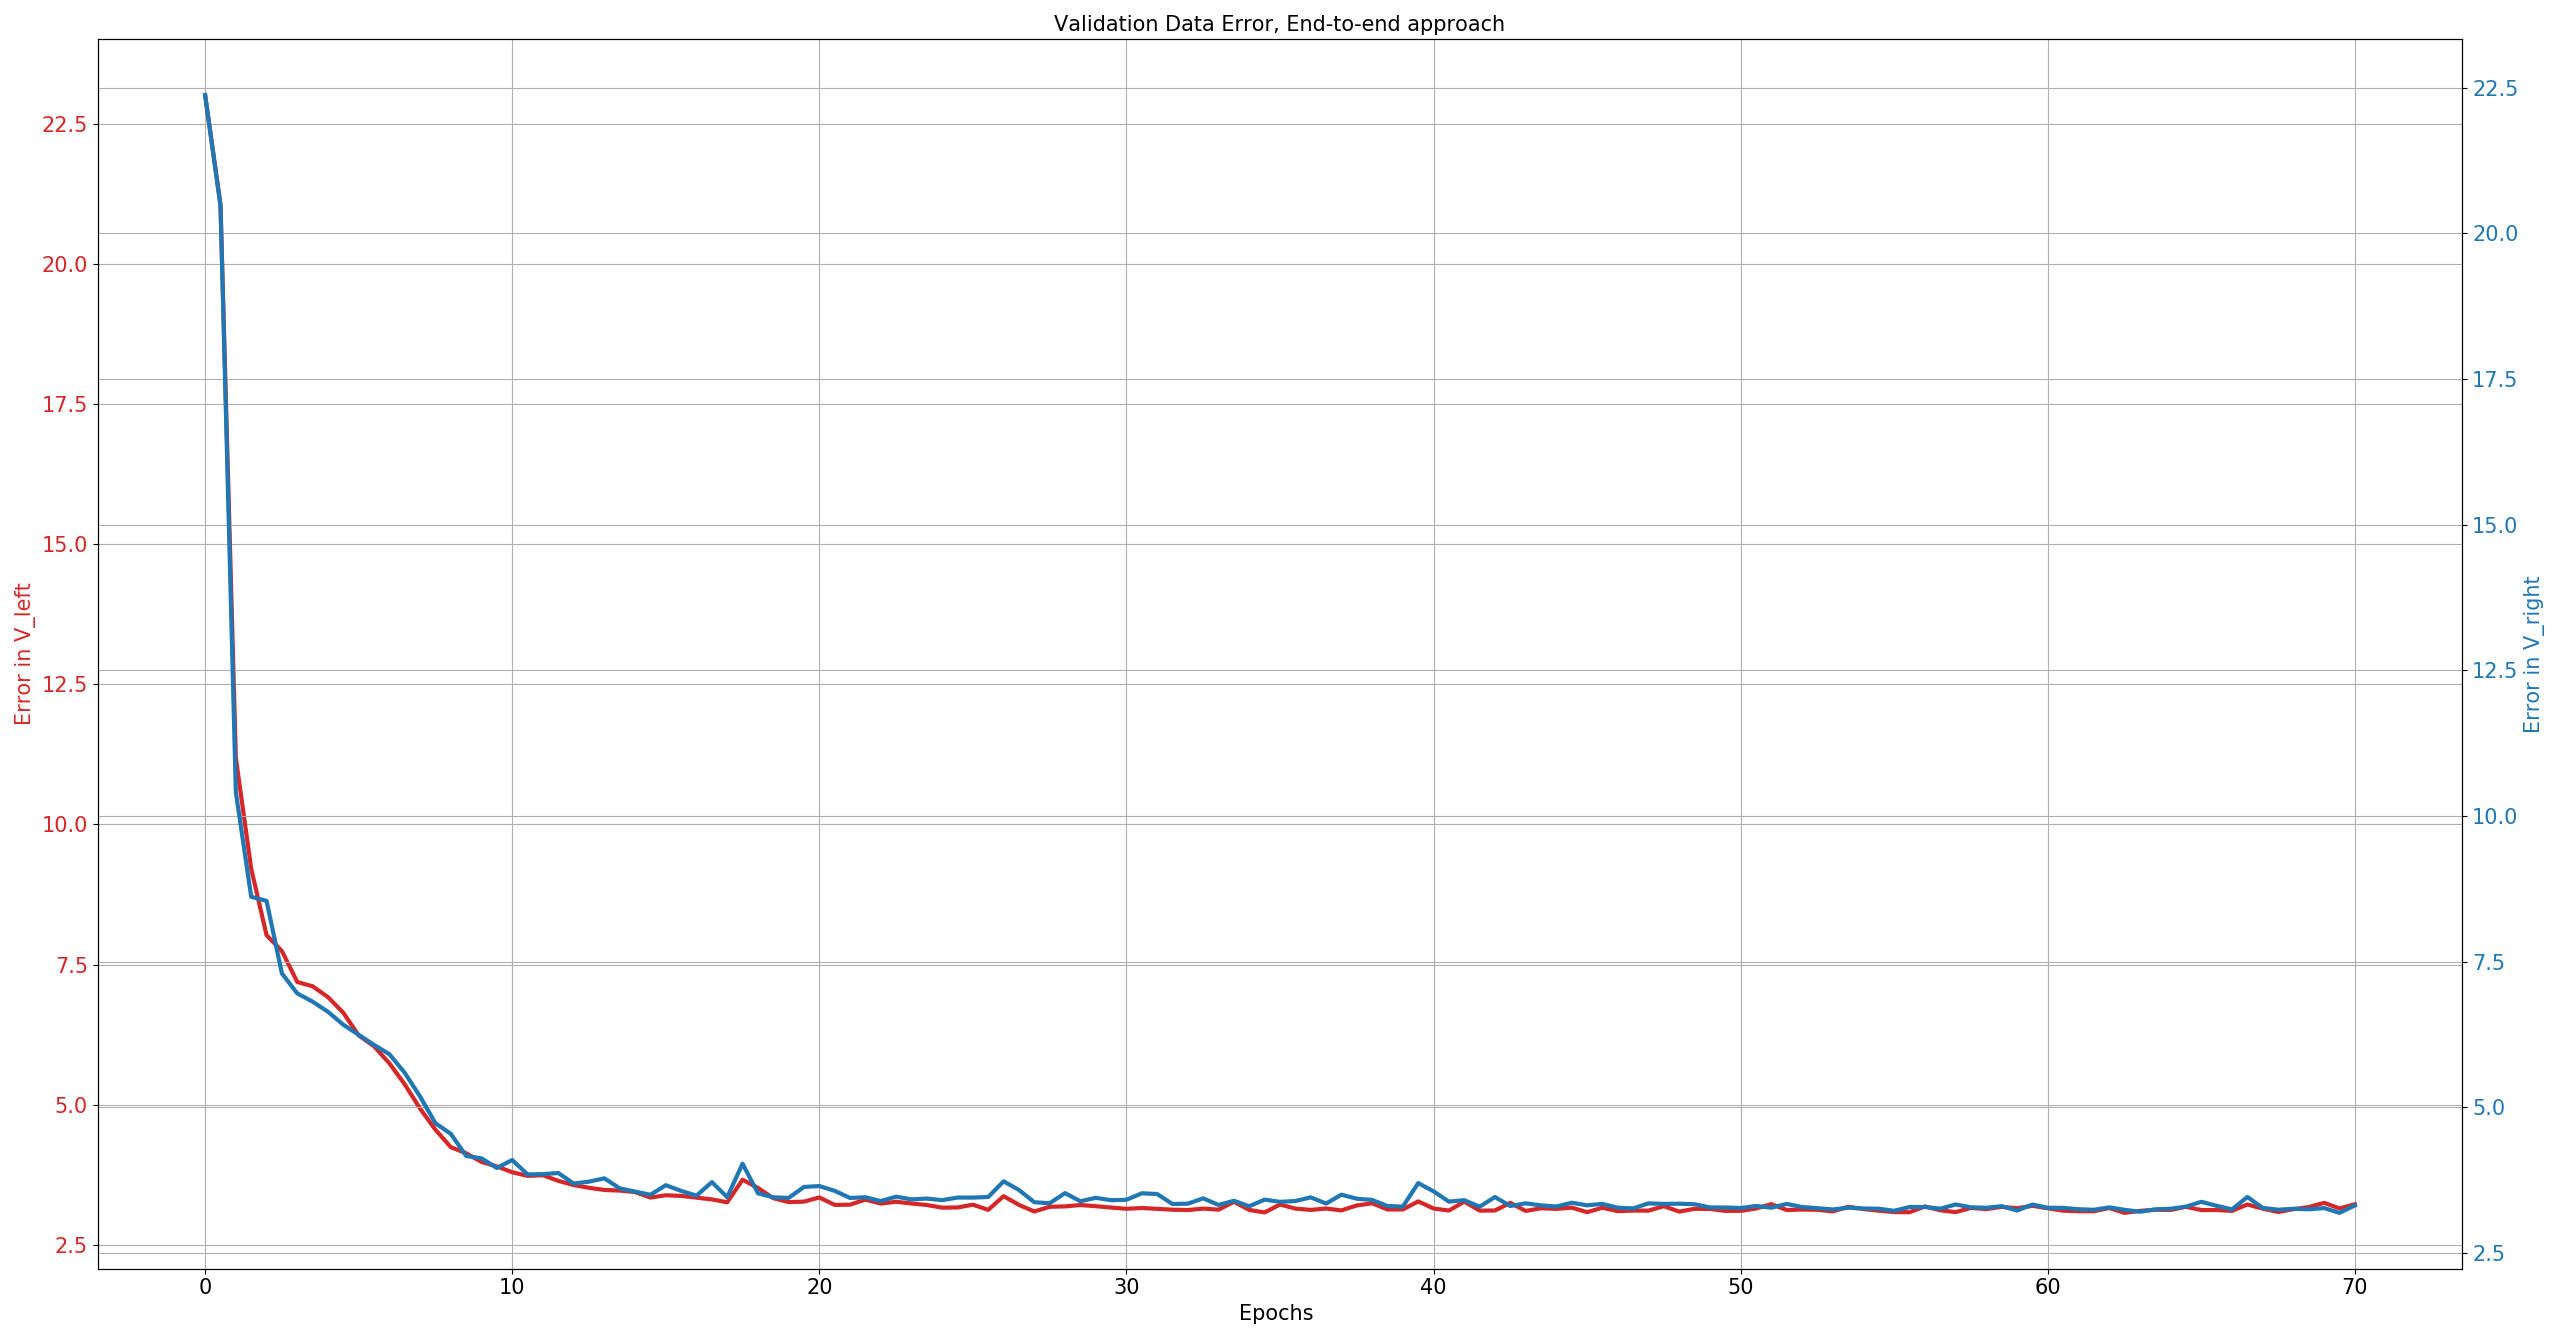
\includegraphics[width=\linewidth]{err-app2.png}
			\caption{Errors wrt. Epochs}
		\end{subfigure}
		\begin{subfigure}[b]{0.14\linewidth}
			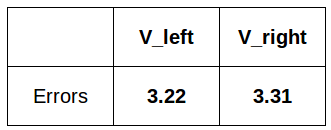
\includegraphics[width=\linewidth]{err-app2-table.png}
			\caption{Resulted Errors}
		\end{subfigure}
		\caption{Validation Data Errors with Training Approach 2}
		\label{fig:12}
	\end{figure}  
	
	\subsubsection{Approach 2: Timing Results}
	Overall timing results can be seen at Figure \ref{fig:13}. Since our new approach eliminates simple steps as well, we observed a small improvement in time relative to best timing performance of previous approach.
	
	\begin{figure}[h!]
		\centering
		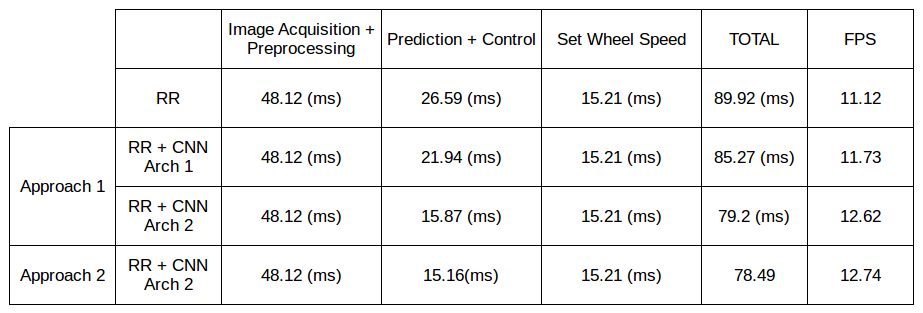
\includegraphics[width=1.0\linewidth]{time-app2.png}
		\caption{Timing Performances.}
		\label{fig:13}
	\end{figure}
	
	\subsection{Real World Experimentation with Training Approach 2 and Conclusions}
	End-to-end approach showed a observable lane following real world performance which can be seen in \href{https://drive.google.com/file/d/1u33WT1eea_rxKjEXIq8q4wmsIBjfPQ2j/view}{here}. When we compare the Deep Learning accuracy of lane following with \href{https://drive.google.com/file/d/1DMLMCO07k4usQVzBTlmiVjwAEVyVyUsn/view}{RR} and \href{https://drive.google.com/file/d/1az6OiYe3fVE5hZonRk_faW_kjZ-aC5JW/view}{ROS}, we observe that Deep Learning approach did not perform as accurate as explicitly implemented algorithms. The further improvements can be achieved with rummaging the data and remove noisy or wrongly labeled images or finding a better CNN architecture.
	
\end{document}